\documentclass[11pt,a4paper]{article}
\usepackage[utf8]{inputenc}
\usepackage[T1]{fontenc}
\usepackage{lmodern}
\usepackage[margin=2.5cm]{geometry}
\usepackage{amsmath,amssymb}
\usepackage{graphicx}
\usepackage{booktabs}
\usepackage[numbers,sort&compress]{natbib}
\usepackage[hidelinks]{hyperref}
\usepackage{url}
\Urlmuskip=0mu plus 1mu
\usepackage{caption}
\captionsetup{font=small,labelfont=bf}
\usepackage{microtype}

% Auto-generated by src/summary.py from results/*.json. Do not edit by hand.
\newcommand{\MlFixHaikuEightyNeu}{0.00}
\newcommand{\MlFixHaikuEightySel}{0.50}
\newcommand{\MlFixHaikuFiveNeu}{0.00}
\newcommand{\MlFixHaikuFiveSel}{0.00}
\newcommand{\MlFixHaikuHalfNeu}{0.00}
\newcommand{\MlFixHaikuHalfSel}{0.20}
\newcommand{\MlFixHaikuTwentyNeu}{0.00}
\newcommand{\MlFixHaikuTwentySel}{0.00}
\newcommand{\MlFixOpusEightyNeu}{0.70}
\newcommand{\MlFixOpusEightySel}{0.80}
\newcommand{\MlFixOpusFiveNeu}{0.05}
\newcommand{\MlFixOpusFiveSel}{0.05}
\newcommand{\MlFixOpusHalfNeu}{0.40}
\newcommand{\MlFixOpusHalfSel}{0.55}
\newcommand{\MlFixOpusTwentyNeu}{0.10}
\newcommand{\MlFixOpusTwentySel}{0.45}
\newcommand{\MlFixSonnetEightyNeu}{0.65}
\newcommand{\MlFixSonnetEightySel}{0.85}
\newcommand{\MlFixSonnetFiveNeu}{0.00}
\newcommand{\MlFixSonnetFiveSel}{0.20}
\newcommand{\MlFixSonnetHalfNeu}{0.15}
\newcommand{\MlFixSonnetHalfSel}{0.70}
\newcommand{\MlFixSonnetTwentyNeu}{0.00}
\newcommand{\MlFixSonnetTwentySel}{0.45}
\newcommand{\MlHendHaikuTen}{0.478}
\newcommand{\MlHendHaikuFifty}{0.487}
\newcommand{\MlHendOpusTen}{0.093}
\newcommand{\MlHendOpusFifty}{0.389}
\newcommand{\MlHendSonnetTen}{0.189}
\newcommand{\MlHendSonnetFifty}{0.385}
\newcommand{\MlLagHaikuTen}{-0.03}
\newcommand{\MlLagHaikuFifty}{-0.10}
\newcommand{\MlLagOpusTen}{-0.03}
\newcommand{\MlLagOpusFifty}{-0.12}
\newcommand{\MlLagSonnetTen}{0.06}
\newcommand{\MlLagSonnetFifty}{0.05}
\newcommand{\MlNeHaikuTen}{4.59}
\newcommand{\MlNeHaikuFifty}{3.46}
\newcommand{\MlNeOpusTen}{1.65}
\newcommand{\MlNeOpusFifty}{1.28}
\newcommand{\MlNeSonnetTen}{3.56}
\newcommand{\MlNeSonnetFifty}{2.97}
\newcommand{\MlPhiMidHaiku}{0.19}
\newcommand{\MlPhiMidOpus}{0.64}
\newcommand{\MlPhiMidSonnet}{0.26}
\newcommand{\MlPullHaikuTen}{-0.027}
\newcommand{\MlPullHaikuFifty}{-0.081}
\newcommand{\MlPullOpusTen}{0.005}
\newcommand{\MlPullOpusFifty}{0.002}
\newcommand{\MlPullSonnetTen}{0.019}
\newcommand{\MlPullSonnetFifty}{0.027}
\newcommand{\MlRevHaikuTen}{0.51}
\newcommand{\MlRevHaikuFifty}{0.54}
\newcommand{\MlRevOpusTen}{0.46}
\newcommand{\MlRevOpusFifty}{0.56}
\newcommand{\MlRevSonnetTen}{0.48}
\newcommand{\MlRevSonnetFifty}{0.48}
\newcommand{\MlSeffHaiku}{0.045}
\newcommand{\MlSeffOpus}{0.052}
\newcommand{\MlSeffSonnet}{0.065}
\newcommand{\WhFixHaikuEightyNeu}{0.25}
\newcommand{\WhFixHaikuEightySel}{0.83}
\newcommand{\WhFixHaikuFiveNeu}{0.33}
\newcommand{\WhFixHaikuFiveSel}{0.42}
\newcommand{\WhFixHaikuHalfNeu}{0.33}
\newcommand{\WhFixHaikuHalfSel}{0.62}
\newcommand{\WhFixHaikuTwentyNeu}{0.25}
\newcommand{\WhFixHaikuTwentySel}{0.42}
\newcommand{\WhFixOpusEightyNeu}{0.75}
\newcommand{\WhFixOpusEightySel}{0.92}
\newcommand{\WhFixOpusFiveNeu}{0.25}
\newcommand{\WhFixOpusFiveSel}{0.25}
\newcommand{\WhFixOpusHalfNeu}{0.50}
\newcommand{\WhFixOpusHalfSel}{0.75}
\newcommand{\WhFixOpusTwentyNeu}{0.25}
\newcommand{\WhFixOpusTwentySel}{0.33}
\newcommand{\WhFixSonnetEightyNeu}{0.67}
\newcommand{\WhFixSonnetEightySel}{0.75}
\newcommand{\WhFixSonnetFiveNeu}{0.33}
\newcommand{\WhFixSonnetFiveSel}{0.25}
\newcommand{\WhFixSonnetHalfNeu}{0.42}
\newcommand{\WhFixSonnetHalfSel}{0.67}
\newcommand{\WhFixSonnetTwentyNeu}{0.33}
\newcommand{\WhFixSonnetTwentySel}{0.50}
\newcommand{\WhHendHaikuTen}{0.082}
\newcommand{\WhHendHaikuFifty}{0.204}
\newcommand{\WhHendOpusTen}{0.067}
\newcommand{\WhHendOpusFifty}{0.307}
\newcommand{\WhHendSonnetTen}{0.079}
\newcommand{\WhHendSonnetFifty}{0.219}
\newcommand{\WhLagHaikuTen}{0.10}
\newcommand{\WhLagHaikuFifty}{0.03}
\newcommand{\WhLagOpusTen}{-0.29}
\newcommand{\WhLagOpusFifty}{-0.25}
\newcommand{\WhLagSonnetTen}{-0.17}
\newcommand{\WhLagSonnetFifty}{-0.09}
\newcommand{\WhNeHaikuTen}{2.18}
\newcommand{\WhNeHaikuFifty}{2.01}
\newcommand{\WhNeOpusTen}{1.16}
\newcommand{\WhNeOpusFifty}{1.31}
\newcommand{\WhNeSonnetTen}{1.44}
\newcommand{\WhNeSonnetFifty}{1.80}
\newcommand{\WhPullHaikuTen}{-0.000}
\newcommand{\WhPullHaikuFifty}{0.040}
\newcommand{\WhPullOpusTen}{0.003}
\newcommand{\WhPullOpusFifty}{0.024}
\newcommand{\WhPullSonnetTen}{0.006}
\newcommand{\WhPullSonnetFifty}{0.040}
\newcommand{\WhRevHaikuTen}{0.41}
\newcommand{\WhRevHaikuFifty}{0.52}
\newcommand{\WhRevOpusTen}{0.68}
\newcommand{\WhRevOpusFifty}{0.65}
\newcommand{\WhRevSonnetTen}{0.61}
\newcommand{\WhRevSonnetFifty}{0.60}
\newcommand{\WhSeffHaiku}{0.072}
\newcommand{\WhSeffOpus}{0.069}
\newcommand{\WhSeffSonnet}{0.064}
\newcommand{\bitsHaikuAlt}{0.638}
\newcommand{\bitsHaikuFreq}{0.511}
\newcommand{\bitsHaikuH}{0.886}
\newcommand{\bitsHaikuMaxrun}{7}
\newcommand{\bitsHaikuRho}{-0.28}
\newcommand{\bitsHaikuRun}{1.60}
\newcommand{\bitsOpusAlt}{0.615}
\newcommand{\bitsOpusFreq}{0.514}
\newcommand{\bitsOpusH}{0.934}
\newcommand{\bitsOpusMaxrun}{4}
\newcommand{\bitsOpusRho}{-0.23}
\newcommand{\bitsOpusRun}{1.67}
\newcommand{\bitsSonnetAlt}{0.664}
\newcommand{\bitsSonnetFreq}{0.509}
\newcommand{\bitsSonnetH}{0.825}
\newcommand{\bitsSonnetMaxrun}{3}
\newcommand{\bitsSonnetRho}{-0.33}
\newcommand{\bitsSonnetRun}{1.53}
\newcommand{\btwHaiku}{0.017}
\newcommand{\btwOpus}{0.001}
\newcommand{\btwSonnet}{0.003}
\newcommand{\ctxTokensM}{83}
\newcommand{\dNeHaikuTen}{1.21}
\newcommand{\dNeHaikuTenHi}{1.36}
\newcommand{\dNeHaikuTenLo}{1.14}
\newcommand{\dNeHaikuTwoHundred}{1.53}
\newcommand{\dNeHaikuTwoHundredHi}{1.65}
\newcommand{\dNeHaikuTwoHundredLo}{1.43}
\newcommand{\dNeHaikuFifty}{1.52}
\newcommand{\dNeHaikuFiftyHi}{1.60}
\newcommand{\dNeHaikuFiftyLo}{1.45}
\newcommand{\dNeHaikuFiftyPlain}{1.59}
\newcommand{\dNeHaikuFiftyRng}{1.52}
\newcommand{\dNeHaikuFiftyWf}{1.46}
\newcommand{\dNeMax}{1.53}
\newcommand{\dNeMin}{1.04}
\newcommand{\dNeOpusTen}{1.18}
\newcommand{\dNeOpusTenHi}{1.21}
\newcommand{\dNeOpusTenLo}{1.15}
\newcommand{\dNeOpusTwoHundred}{1.04}
\newcommand{\dNeOpusTwoHundredHi}{1.08}
\newcommand{\dNeOpusTwoHundredLo}{1.01}
\newcommand{\dNeOpusFifty}{1.06}
\newcommand{\dNeOpusFiftyHi}{1.08}
\newcommand{\dNeOpusFiftyLo}{1.03}
\newcommand{\dNeOpusFiftyPlain}{1.11}
\newcommand{\dNeOpusFiftyRng}{1.08}
\newcommand{\dNeOpusFiftyWf}{1.01}
\newcommand{\dNeSonnetTen}{1.09}
\newcommand{\dNeSonnetTenHi}{1.12}
\newcommand{\dNeSonnetTenLo}{1.06}
\newcommand{\dNeSonnetTwoHundred}{1.52}
\newcommand{\dNeSonnetTwoHundredHi}{1.60}
\newcommand{\dNeSonnetTwoHundredLo}{1.45}
\newcommand{\dNeSonnetFifty}{1.46}
\newcommand{\dNeSonnetFiftyHi}{1.53}
\newcommand{\dNeSonnetFiftyLo}{1.40}
\newcommand{\dNeSonnetFiftyPlain}{1.40}
\newcommand{\dNeSonnetFiftyRng}{1.19}
\newcommand{\dNeSonnetFiftyWf}{1.53}
\newcommand{\dSeffHaikuTen}{0.016}
\newcommand{\dSeffHaikuTwoHundred}{0.043}
\newcommand{\dSeffHaikuFifty}{0.032}
\newcommand{\dSeffOpusTen}{0.046}
\newcommand{\dSeffOpusTwoHundred}{0.051}
\newcommand{\dSeffOpusFifty}{0.041}
\newcommand{\dSeffSonnetTen}{0.104}
\newcommand{\dSeffSonnetTwoHundred}{0.054}
\newcommand{\dSeffSonnetFifty}{0.076}
\newcommand{\dupAgreeHaiku}{0.16}
\newcommand{\dupAgreeOpus}{0.43}
\newcommand{\dupAgreeSonnet}{0.34}
\newcommand{\dupPrefixHaiku}{4.5}
\newcommand{\dupPrefixOpus}{18.2}
\newcommand{\dupPrefixSonnet}{4.2}
\newcommand{\exactMeanExp}{0.09}
\newcommand{\exactMeanHaiku}{0.12}
\newcommand{\exactMeanOpus}{0.11}
\newcommand{\exactMeanSonnet}{0.13}
\newcommand{\fcFixedHaiku}{0}
\newcommand{\fcFixedOpus}{0}
\newcommand{\fcFixedSonnet}{0}
\newcommand{\fcNHaiku}{8}
\newcommand{\fcNOpus}{12}
\newcommand{\fcNSonnet}{8}
\newcommand{\fcNeHaiku}{3.3}
\newcommand{\fcNeOpus}{3.7}
\newcommand{\fcNeSonnet}{3.5}
\newcommand{\fcSurFixHaiku}{0.19}
\newcommand{\fcSurFixOpus}{0.15}
\newcommand{\fcSurFixSonnet}{0.24}
\newcommand{\fcSurNeHaiku}{1.38}
\newcommand{\fcSurNeOpus}{1.28}
\newcommand{\fcSurNeSonnet}{1.45}
\newcommand{\fcTHaiku}{31}
\newcommand{\fcTOpus}{22}
\newcommand{\fcTSonnet}{32}
\newcommand{\freqHaikuEighty}{0.873}
\newcommand{\freqHaikuFive}{0.025}
\newcommand{\freqHaikuTwenty}{0.105}
\newcommand{\freqOpusEighty}{0.828}
\newcommand{\freqOpusFive}{0.024}
\newcommand{\freqOpusTwenty}{0.158}
\newcommand{\freqSonnetEighty}{0.819}
\newcommand{\freqSonnetFive}{0.023}
\newcommand{\freqSonnetTwenty}{0.140}
\newcommand{\iidMaxRun}{8}
\newcommand{\lagDrawHaiku}{-0.44}
\newcommand{\lagDrawOpus}{-0.33}
\newcommand{\lagDrawSonnet}{-0.37}
\newcommand{\lenExactHaiku}{0}
\newcommand{\lenExactOpus}{33}
\newcommand{\lenExactSonnet}{2}
\newcommand{\lenMaxHaiku}{3816}
\newcommand{\lenMaxOpus}{348}
\newcommand{\lenMaxSonnet}{402}
\newcommand{\lenMinHaiku}{174}
\newcommand{\lenMinOpus}{288}
\newcommand{\lenMinSonnet}{243}
\newcommand{\markovUnderFactor}{8}
\newcommand{\maxAbsBias}{0.042}
\newcommand{\medAbsBias}{0.0013}
\newcommand{\mfiveExp}{0.20}
\newcommand{\mfiveObs}{0.21}
\newcommand{\mlRetries}{0}
\newcommand{\nCalls}{1,193}
\newcommand{\nCallsHaiku}{433}
\newcommand{\nCallsOpus}{381}
\newcommand{\nCallsSonnet}{379}
\newcommand{\nDirectDraws}{6,720}
\newcommand{\nFull}{1,163}
\newcommand{\nFullBits}{264}
\newcommand{\nFullBitsdup}{12}
\newcommand{\nFullDirect}{324}
\newcommand{\nFullDirectdup}{12}
\newcommand{\nFullMl}{464}
\newcommand{\nFullTraj}{87}
\newcommand{\nInvalidDirect}{0}
\newcommand{\nOtherTools}{0}
\newcommand{\nPilot}{30}
\newcommand{\nPilotBits}{9}
\newcommand{\nPilotDirect}{12}
\newcommand{\nPilotMl}{6}
\newcommand{\nPilotTraj}{3}
\newcommand{\nValid}{1,193}
\newcommand{\nWhTraj}{344}
\newcommand{\npFixEightyNeu}{0.74}
\newcommand{\npFixEightySel}{0.88}
\newcommand{\npFixFiveNeu}{0.03}
\newcommand{\npFixFiveSel}{0.08}
\newcommand{\npFixHalfNeu}{0.41}
\newcommand{\npFixHalfSel}{0.62}
\newcommand{\npFixTwentyNeu}{0.14}
\newcommand{\npFixTwentySel}{0.28}
\newcommand{\npHendFifty}{0.369}
\newcommand{\npHendTen}{0.065}
\newcommand{\npRevTen}{0.49}
\newcommand{\phiFirstHaiku}{0.09}
\newcommand{\phiFirstOpus}{0.10}
\newcommand{\phiFirstSonnet}{0.10}
\newcommand{\phiLaterHaiku}{0.70}
\newcommand{\phiLaterOpus}{0.96}
\newcommand{\phiLaterSonnet}{0.78}
\newcommand{\prefixHaiku}{4.2}
\newcommand{\prefixOpus}{21.7}
\newcommand{\prefixSonnet}{9.3}
\newcommand{\repFirstThree}{0.36}
\newcommand{\rhoFourHaiku}{-0.20}
\newcommand{\rhoFourOpus}{-0.27}
\newcommand{\rhoFourSonnet}{-0.27}
\newcommand{\rhoThreeHaiku}{0.07}
\newcommand{\rhoThreeOpus}{-0.00}
\newcommand{\rhoThreeSonnet}{0.16}
\newcommand{\rngAcfHaikuFive}{1.9}
\newcommand{\rngAcfHaikuHalf}{7.2}
\newcommand{\rngAcfHaikuTwenty}{1.5}
\newcommand{\rngAcfMaxDev}{21}
\newcommand{\rngAcfOpusFive}{3.9}
\newcommand{\rngAcfOpusHalf}{12.8}
\newcommand{\rngAcfOpusTwenty}{8.5}
\newcommand{\rngAcfSonnetFive}{3.9}
\newcommand{\rngAcfSonnetHalf}{13.9}
\newcommand{\rngAcfSonnetTwenty}{10.3}
\newcommand{\rngMarkovHaikuFive}{2.1}
\newcommand{\rngMarkovHaikuHalf}{1.7}
\newcommand{\rngMarkovHaikuTwenty}{2.1}
\newcommand{\rngMarkovOpusFive}{2.1}
\newcommand{\rngMarkovOpusHalf}{1.6}
\newcommand{\rngMarkovOpusTwenty}{1.4}
\newcommand{\rngMarkovSonnetFive}{2.2}
\newcommand{\rngMarkovSonnetHalf}{1.9}
\newcommand{\rngMarkovSonnetTwenty}{1.8}
\newcommand{\rngNeHaikuFive}{1.9}
\newcommand{\rngNeHaikuHalf}{6.5}
\newcommand{\rngNeHaikuHalfFifty}{9.2}
\newcommand{\rngNeHaikuTwenty}{1.5}
\newcommand{\rngNeMax}{13.9}
\newcommand{\rngNeMin}{6.5}
\newcommand{\rngNeOpusFive}{3.8}
\newcommand{\rngNeOpusHalf}{12.7}
\newcommand{\rngNeOpusHalfFifty}{33.2}
\newcommand{\rngNeOpusTwenty}{7.3}
\newcommand{\rngNeSonnetFive}{3.8}
\newcommand{\rngNeSonnetHalf}{13.9}
\newcommand{\rngNeSonnetHalfFifty}{28.6}
\newcommand{\rngNeSonnetTwenty}{8.5}
\newcommand{\sTrueApprox}{0.049}
\newcommand{\secsHaiku}{4.6}
\newcommand{\secsOpus}{3.9}
\newcommand{\secsSonnet}{3.3}
\newcommand{\slopeHaiku}{1.32}
\newcommand{\slopeHaikuHi}{1.45}
\newcommand{\slopeHaikuLo}{1.22}
\newcommand{\slopeOpus}{1.22}
\newcommand{\slopeOpusHi}{1.24}
\newcommand{\slopeOpusLo}{1.20}
\newcommand{\slopeSonnet}{1.23}
\newcommand{\slopeSonnetHi}{1.25}
\newcommand{\slopeSonnetLo}{1.21}
\newcommand{\thMaxNeErr}{1.5}
\newcommand{\thMaxVarErr}{2.1}
\newcommand{\topFirstHaiku}{4}
\newcommand{\topFirstOpus}{13}
\newcommand{\topFirstSonnet}{9}
\newcommand{\trajNeMax}{4.6}
\newcommand{\trajNeMin}{1.2}
\newcommand{\wfTabsTen}{27.7}
\newcommand{\whBadLength}{7}
\newcommand{\whBadNumber}{1}
\newcommand{\whLeftBoundary}{0}
\newcommand{\whSexMax}{47}
\newcommand{\whSexMin}{32}
\newcommand{\withinExp}{0.66}
\newcommand{\withinHaiku}{0.74}
\newcommand{\withinOpus}{0.66}
\newcommand{\withinSonnet}{0.72}

\newcommand{\Ne}{N_e}
\newcommand{\Var}{\operatorname{Var}}
\newcommand{\E}{\operatorname{E}}

\title{Can a language model be random enough to be evolution?\\
\large Genetic drift with a large language model as the random number source}
\author{Sara Behnamian\\
\small Department of Biology, Lund University, Sweden\\
\small \texttt{sara.behnamian@biol.lu.se}}
\date{}

\begin{document}
\maketitle

\begin{abstract}
Genetic drift is sampling noise: in the Wright--Fisher model the next generation's allele count is a binomial draw.
Large language models (LLMs) are increasingly used inside simulations and agent-based models, and they are known to produce ``random'' output with human-like biases.
We asked what happens to drift when an LLM supplies the randomness, and expressed the answer in population-genetic units, as the variance effective population size $\Ne$ implied by the LLM's sampling.
Using \nCalls{} independent calls to three models of one family (Haiku, Sonnet and Opus), we measured raw bit sequences, single-generation Wright--Fisher draws, multi-generation trajectories built from one fresh call per generation or from one call per whole trajectory, and an ``RNG mode'' in which LLM bits drive an otherwise exact simulation.
All three models over-alternated (alternation rate \bitsOpusAlt--\bitsSonnetAlt{} against 0.5) and exaggerated requested probabilities rather than shrinking them toward one half (logit slope \slopeOpus--\slopeHaiku).
When asked for the next generation directly, the models got the mean right but the variance too small: $\Ne/N$ was \dNeOpusTwoHundred--\dNeHaikuTwoHundred{} at $N=200$.
In multi-generation runs the excess was larger, up to $\Ne/N=\MlNeHaikuTen$ (Haiku, one call per generation), so heterozygosity decayed too slowly and alleles fixed too late.
Used as a bit source, LLM output was so locally balanced that $\Ne/N$ reached \rngNeSonnetHalf{} for $N=10$, far more than a first-order Markov model of the alternation bias predicts; the full autocorrelation function accounts for it.
The direction of selection was respected, and in whole-trajectory runs its effect was exaggerated (effective $s$ \WhSeffSonnet--\WhSeffHaiku{} for a stated $s=0.05$).
The largest model was the closest to Wright--Fisher behaviour in every direct mode, but its raw bits were no better than those of the smaller models and were the most repetitive across calls.
LLM-generated randomness is therefore a poor substitute for a pseudo-random number generator in evolutionary models: it makes drift too weak, and the size of the error depends on model, prompt and how calls are batched.
\end{abstract}

\section{Introduction}

Genetic drift is the change in allele frequencies caused by the random sampling of gametes in a finite population \citep{wright1931evolution,fisher1930genetical}.
In the Wright--Fisher (WF) model, a diploid population of $N$ individuals carries $2N$ gene copies, and given an allele frequency $p$ the next generation's count of that allele is Binomial$(2N,p)$.
The variance of the change, $\Var(\Delta p)=p(1-p)/2N$, sets the pace of everything that follows: heterozygosity decays by a factor $1-1/2N$ per generation, a neutral allele fixes with probability equal to its starting frequency, and absorption takes on the order of $4N$ generations \citep{kimura1962probability,kimura1969average,ewens2004mathematical}.
Real populations rarely match the idealised model, so population geneticists describe them by an effective size $\Ne$, the size of an ideal WF population with the same rate of drift \citep{crow1970introduction,charlesworth2009effective}.

The quality of the randomness matters for simulation.
Pseudo-random number generators are tested with large statistical batteries \citep{lecuyer2007testu01}, and subtle correlations in a generator that passed common tests have produced wrong answers in Monte Carlo physics \citep{ferrenberg1992monte}.
At the same time, LLMs are being placed inside simulations: as agents in social sandboxes \citep{park2023generative}, as simulated economic actors or survey respondents \citep{horton2023large,argyle2023out,aher2023using}, in agent-based models more broadly \citep{gao2024large}, and as mutation or crossover operators in evolutionary computation \citep{lehman2022evolution,meyerson2024language}.
In such systems an LLM is often the only source of stochastic behaviour.
If it is asked to ``simulate'' a random process, its sampling errors become part of the model.

It is already well established that LLMs are poor random generators.
Asked to flip coins, models reproduce and amplify human biases: too much alternation, too few long runs and too many balanced sequences \citep{koevering2024random}.
Asked for random numbers, they favour a few values \citep{zhang2024forcing,coronado2025deterministic}, avoid repeats and neighbouring numbers \citep{harrison2024comparison}, and fail to match target distributions in batch and stateless settings \citep{hopkins2023random,gu2025dice,zhao2026dice,gu2026stochasticity,karanjai2025randomness}.
Biased coins come out biased in the wrong way \citep{xiao2025flipping,gupta2025coinflips}, and models do not randomise well in games \citep{guo2025illusion,yang2025flipcoin}.
These patterns echo the human literature: people over-alternate, expect small samples to be representative, and see streaks where there are none \citep{wagenaar1972generation,tversky1971belief,gilovich1985hot,barhillel1991perception,falk1997making,rapoport1992generation}, although the strength of the human deficit depends on the task \citep{nickerson2002production}.

What has not been done is to follow these biases into a stochastic model whose output depends on them in a known way.
Genetic drift is a natural test case because its theory is exact, and because its central quantity, the variance of a binomial draw, is exactly what biased random generation distorts.
Our contribution is to express LLM randomness in population-genetic units.
We (i) quantify bias, alternation, run lengths and probability distortion in LLM bit sequences, (ii) ask LLMs to carry out WF sampling directly and estimate $\Ne/N$, (iii) run multi-generation trajectories with and without memory and compare heterozygosity decay, fixation probability, absorption time and the response to selection with exact theory and a numpy baseline, (iv) feed LLM bits into an otherwise exact WF simulation (``RNG mode'') to separate bad randomness from a poor model of the process, and (v) compare three model sizes.
A short theory section links simple parametric models of LLM randomness to $\Ne$, heterozygosity and fixation.

\section{Theory}
\label{sec:theory}

Full derivations are in \texttt{theory/derivations.md}, and the script \texttt{theory/check\_theory.py} checks them numerically.
For any process that maps $p$ to $p+\Delta p$, we use the variance effective size
\begin{equation}
\Ne = \frac{p(1-p)}{2\Var(\Delta p\mid p)}, \label{eq:ne}
\end{equation}
so that $\Ne=N$ for exact WF. $\Ne/N>1$ means drift is too slow.

\paragraph{Bit sequences.}
We model LLM bits $b_1,b_2,\dots$ requested with probability $p$ as a stationary two-state Markov chain with produced frequency $\pi$ and lag-1 autocorrelation $\rho$ ($\rho<0$: excess alternation).
Then the alternation rate is $2\pi(1-\pi)(1-\rho)$, runs of ones are geometric with continuation probability $\pi+\rho(1-\pi)$, and the sum of $n$ bits has variance
\begin{equation}
\Var(S_n)= n\pi(1-\pi)\left[\frac{1+\rho}{1-\rho}-\frac{2\rho(1-\rho^n)}{n(1-\rho)^2}\right]. \label{eq:markov}
\end{equation}
The distortion of the requested probability is summarised by a logit-linear curve, $\operatorname{logit}\pi=\beta_0+\beta_1\operatorname{logit}p$; $\beta_1<1$ is shrinkage toward one half and $\beta_1>1$ is exaggeration.

\paragraph{RNG mode.}
If each of the $2N$ offspring copies inherits allele $A$ when its LLM bit is 1, with bits requested at the current $p$, then $\E[\Delta p]=\pi-p$ and, from \eqref{eq:markov},
\begin{equation}
\frac{\Ne}{N}\approx \frac{p(1-p)}{\pi(1-\pi)}\cdot\frac{1-\rho}{1+\rho}. \label{eq:rng}
\end{equation}
Excess alternation slows drift ($\rho=-0.2$ gives $\Ne/N\approx1.5$).
The first-order chain is only a model; more generally $\Var(S_n)=\sum_{i,j}\gamma_{|i-j|}$ with $\gamma_k$ the lag-$k$ autocovariance, and we evaluate both forms against data.
Exaggeration ($\beta_1>1$) adds a systematic $\E[\Delta p]$ that pushes frequencies away from one half, toward the nearest boundary.

\paragraph{Direct mode.}
When an LLM produces next-generation counts, we describe them by a conditional mean $m(p)$ and a dispersion factor $\phi$, with $\Var(X\mid p)=\phi\,2N\,m(1-m)$.
Then $\Ne/N=p(1-p)/(\phi\,m(1-m))\approx1/\phi$ when $m\approx p$.
If the mean is unbiased, heterozygosity $H=2p(1-p)$ obeys
\begin{equation}
\E[H_t]=H_0\left(1-\frac{\phi}{2N}\right)^t=H_0\left(1-\frac{1}{2\Ne}\right)^t . \label{eq:het}
\end{equation}
With drift $M(p)=m(p)-p$ and variance $V(p)=\phi p(1-p)/2N$, the diffusion fixation probability is $u(p_0)=\int_0^{p_0}G/\int_0^1G$ with $G(x)=\exp(-\int 2M/V)$.
Two consequences follow.
First, if $M=0$, then $u(p_0)=p_0$ whatever $\phi$ is: dispersion errors alone leave neutral fixation probabilities unchanged and only slow the process; the mean time to absorption, $-4\Ne[p_0\ln p_0+(1-p_0)\ln(1-p_0)]$, scales with $\Ne$ \citep{kimura1969average}.
Second, if selection is represented as $M=s_{\mathrm{eff}}\,p(1-p)$, Kimura's result becomes
\begin{equation}
u(p_0)=\frac{1-e^{-4\Ne s_{\mathrm{eff}} p_0}}{1-e^{-4\Ne s_{\mathrm{eff}}}}, \label{eq:kimura}
\end{equation}
so an LLM that gets $s$ right but has $\Ne/N>1$ still exaggerates the effect of selection, because only the product $\Ne s_{\mathrm{eff}}$ matters \citep{kimura1962probability}.
In whole trajectories with an unbiased conditional mean, successive increments $\Delta p_t$ are uncorrelated; positive correlation means trajectories that are too smooth and negative correlation means too many reversals.

\paragraph{Checks.}
Simulated Markov chains matched \eqref{eq:markov} to within \thMaxVarErr\% and \eqref{eq:rng} to within \thMaxNeErr\%.
Simulations of the dispersion model reproduced \eqref{eq:het}, neutral fixation at $p_0$ for $\phi=0.5$ and $\phi=2$, and \eqref{eq:kimura}; the diffusion results were less accurate for $N=10$ with strong under-dispersion, where count discreteness matters (details in the theory note).

\section{Methods}

\subsection{LLM calls}
No API key was available, so each LLM call was made by a fresh subagent launched by the Claude Code agent harness, using the three model tiers available to subagents (Haiku, Sonnet, Opus).
Each subagent received one prompt and no other context from the experiment, ran at low reasoning effort, and had to return its answer through a structured-output tool validated against a JSON schema (a string of bits, a list of integers, or a list of trajectories).
Every prompt began with the instruction to produce the random output directly and not to write or run code, use other tools, or use any external source of randomness.
We parsed every subagent transcript: in all \nCalls{} calls the only tool used was the structured-output tool (\nOtherTools{} exceptions), and every call returned schema-valid JSON (\nValid{} of \nCalls).
There were no refusals.
Prompts, raw responses, timestamps and the served model family of every call are stored in \texttt{data/raw/calls.jsonl}; the scripts that generated the calls, ingested the transcripts and analysed them are in \texttt{src/}.
All numpy simulations use fixed seeds.
Median wall time per call was \secsSonnet--\secsHaiku{} s.
Because each subagent carries the harness's system prompt, calls consumed about \ctxTokensM{} million input tokens in total, almost all of it cached context; output was small.

Replicate calls of the same condition carried a different six-character ``run code'' (a hash of the call identifier, described as a bookkeeping label), because identical prompts would otherwise invite identical answers.
A separate determinism test repeated two prompts four times each without a run code.

\subsection{Design}
A pilot of \nPilot{} calls checked JSON validity, refusals, timing and output shape across all modes and models.
The full run had \nFull{} calls:
\begin{itemize}
\item \textbf{Bit sequences} (\nFullBits{} calls): 300 bits per call, requested $p\in\{0.05,0.2,0.5,0.8\}$, two phrasings (plain; ``you are a random number generator''), 8 replicates per cell and 20 at $p=0.5$, whose bits also fed RNG mode. We analysed the first 300 digits of each answer and report length errors separately.
\item \textbf{Direct mode, one generation} (\nFullDirect{} calls): 20 next-generation draws per call from a stated state, explicitly required to be independent. Full grid $N\in\{10,50,200\}$, $p\in\{0.05,0.2,0.5,0.8\}$; neutral cells with two phrasings (plain; ``simulate exactly as a Wright--Fisher process'') and three calls each, selection cells ($s=0.05$, WF phrasing) with two calls each, and the third phrasing (random number generator) at $N=50$ only.
\item \textbf{Fresh call per generation} (\nFullMl{} calls): each generation of a set of populations was one new call that saw only the current counts and the generation number. To keep the call count down, up to 40 independent populations were batched in one call. $N=10$ with 20 populations at each $p_0\in\{0.05,0.2,0.5,0.8\}$ for 40 generations, with $s=0$ and $s=0.05$; and $N=50$, 40 populations at $p_0=0.5$, $s=0$, for 30 generations. Absorbed populations were dropped from later calls.
\item \textbf{Whole trajectory per call} (\nFullTraj{} calls): four independent trajectories per call. $N=10$, all four $p_0$, $s\in\{0,0.05\}$, 40 generations, 3 calls per cell; $N=50$, $p_0=0.5$, 30 generations, 5 calls.
\item \textbf{Determinism test} (\nFullBitsdup{}+\nFullDirectdup{} calls).
\end{itemize}
The multi-generation part of the requested grid was trimmed to keep the total near 1,200 calls: trajectories were run only for $N=10$ (all $p_0$, both $s$) and $N=50$ ($p_0=0.5$, $s=0$), and the selection and third-phrasing cells of direct mode have fewer calls.

\subsection{Analysis}
For direct mode we pooled draws within each cell and estimated $\phi=\widehat{\Var}(X/2N)\big/[m(1-m)/2N]$, with $m$ the WF expectation after selection; $\Ne/N=1/\phi$.
Summaries per model and $N$ average $\phi$ over neutral cells (plain and WF phrasings) and invert it.
Confidence intervals come from bootstrapping calls within cells (2,000 resamples for cells, 500 for summaries), which keeps the within-call dependence intact.
For trajectories we estimated $\Ne$ from all transitions starting at polymorphic states, $\hat\Ne=\sum p_t(1-p_t)\big/2\sum(\Delta p_t)^2$, and an effective selection coefficient by regressing $\Delta p$ on $p(1-p)$ through the origin.
For comparison we ran 5,000 numpy WF replicates of every trajectory design, truncated at the same generation, and we report fixation as ``fixed by the last generation'' for LLM and numpy runs alike.
In RNG mode, the bits of each model and requested $p$ were concatenated in call order and cut into non-overlapping windows of $2N$ bits, each window giving one offspring generation.
For a multi-generation version we turned the $p=0.5$ bits into Bernoulli($p$) draws with the standard comparison method (two bits per draw on average) and ran $N=10$ populations from $p_0=0.5$ until the bits ran out; because that gives only a handful of trajectories, we also ran 3,000 trajectories driven by a Markov chain fitted to the same bits.

\section{Results}

\subsection{Raw randomness}

\begin{table}[t]
\centering\small
\caption{Bit sequences requested with $p=0.5$ (pooled phrasings, 40 calls and about 12,000 bits per model), and the slope of the logit shrinkage curve fitted across $p\in\{0.05,0.2,0.5,0.8\}$. The iid row gives the expectation for independent fair bits; the longest run is the median over simulated 300-bit sequences.}
\label{tab:bits}
\resizebox{\textwidth}{!}{\begin{tabular}{lccccccc}
\toprule
Model & freq. of 1s & alternation & $\hat\rho_1$ & mean run & longest run & entropy rate & logit slope $\beta_1$ [95\% CI] \\
\midrule
iid ideal & 0.500 & 0.500 & 0 & 2.00 & 8 (median) & 1.000 & 1 \\
Haiku & 0.511 & 0.638 & -0.28 & 1.60 & 7 & 0.886 & 1.32 [1.22, 1.45] \\
Sonnet & 0.509 & 0.664 & -0.33 & 1.53 & 3 & 0.825 & 1.23 [1.21, 1.25] \\
Opus & 0.514 & 0.615 & -0.23 & 1.67 & 4 & 0.934 & 1.22 [1.20, 1.24] \\
\bottomrule
\end{tabular}
}
\end{table}

At $p=0.5$ all three models produced balanced frequencies but alternated far too often (Table~\ref{tab:bits}): the alternation rate was \bitsOpusAlt{} (Opus), \bitsHaikuAlt{} (Haiku) and \bitsSonnetAlt{} (Sonnet), against 0.5, and the lag-1 autocorrelation was \bitsOpusRho{} to \bitsSonnetRho.
Long runs were missing: the longest run of identical digits in any 300-bit answer was \bitsSonnetMaxrun{} for Sonnet and \bitsOpusMaxrun{} for Opus, where a random sequence of that length typically contains a run of \iidMaxRun{} (Fig.~\ref{fig:runs}).
The dependence was not first-order.
The autocorrelation alternated in sign with lag, with a strong negative value at lag 4 (\rhoFourHaiku{}, \rhoFourSonnet{}, \rhoFourOpus{} for Haiku, Sonnet, Opus) and positive values at lag 3 (Fig.~\ref{fig:dep}a), the signature of short repeating motifs.
Block-entropy estimates of the entropy rate were \bitsSonnetH--\bitsOpusH{} bits per digit.

For other probabilities, the models did not shrink toward one half, as a ``hedging'' model would predict.
They exaggerated (Fig.~\ref{fig:shrink}).
At $p=0.05$ the produced frequency was \freqSonnetFive--\freqHaikuFive, at $p=0.2$ it was \freqHaikuTwenty--\freqOpusTwenty, and at $p=0.8$ it was \freqSonnetEighty--\freqHaikuEighty.
The fitted logit slopes were \slopeOpus{} [\slopeOpusLo, \slopeOpusHi] for Opus, \slopeSonnet{} [\slopeSonnetLo, \slopeSonnetHi] for Sonnet and \slopeHaiku{} [\slopeHaikuLo, \slopeHaikuHi] for Haiku.
Rare outcomes were also spaced too evenly: at $p=0.2$ runs of zeros peaked at four to six instead of decaying geometrically from one (Fig.~\ref{fig:runs}b), and ones almost never appeared in pairs.

Two practical problems are worth noting.
Output length was rarely right: none of Haiku's answers had exactly 300 digits (range \lenMinHaiku--\lenMaxHaiku, with some answers degenerating into long blocks of zeros), against \lenExactOpus\% for Opus.
And calls were not independent of each other even with distinct run codes: pairs of Opus answers at $p=0.5$ shared their first \prefixOpus{} digits on average, and up to \topFirstOpus{} of 20 Opus answers began with the same 16 digits (Sonnet \prefixSonnet, Haiku \prefixHaiku).
Repeating a prompt verbatim gave no exact duplicates, but Opus answers again shared long prefixes (\dupPrefixOpus{} digits on average).

\begin{figure}[t]
\centering
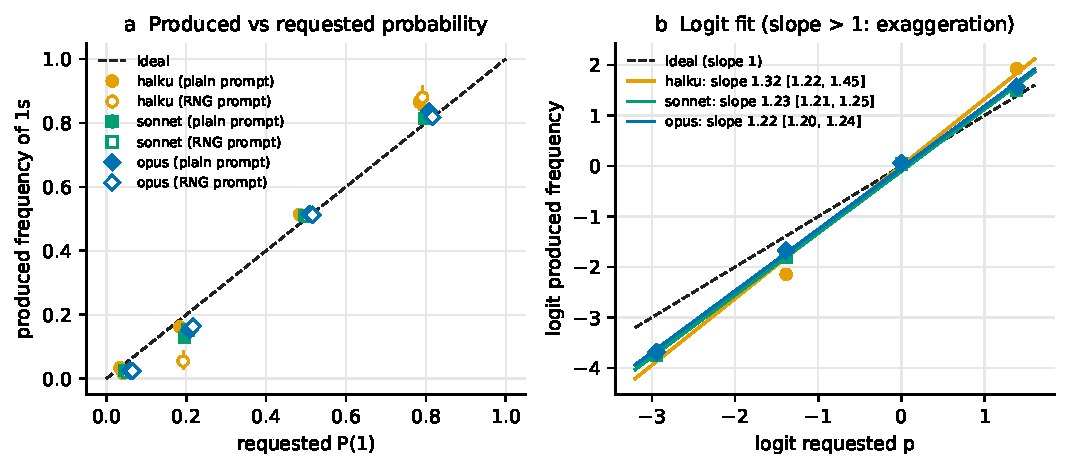
\includegraphics[width=\textwidth]{../figures/fig1_shrinkage.pdf}
\caption{Produced versus requested probability in LLM bit sequences. (a) Pooled frequency of 1s per model and phrasing with 95\% bootstrap intervals over calls. (b) Logit-linear fit; slopes above 1 mean the requested probability is exaggerated, so rare outcomes are under-produced.}
\label{fig:shrink}
\end{figure}

\begin{figure}[t]
\centering
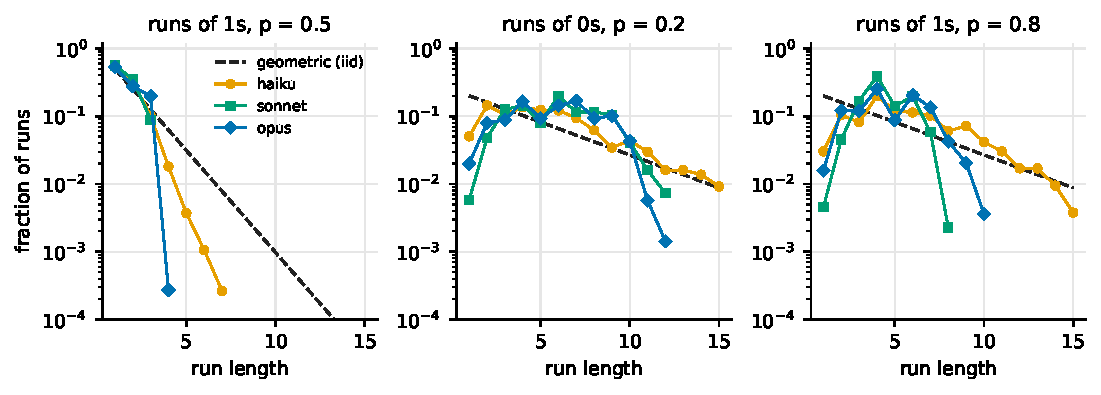
\includegraphics[width=\textwidth]{../figures/fig2_runs.pdf}
\caption{Run-length distributions of LLM bits against the geometric distribution expected for independent bits at the requested probability. Runs are counted within calls.}
\label{fig:runs}
\end{figure}

\subsection{The LLM as the Wright--Fisher process}

\begin{table}[t]
\centering\small
\caption{Effective population size relative to the stated size, $\Ne/N$, by model and mode. Direct mode: neutral cells averaged over $p$ and two phrasings. Trajectory modes: $p_0=0.5$, $s=0$, estimated from all polymorphic transitions. RNG mode: one LLM bit per offspring copy, bits requested at $p=0.5$. Exact WF gives 1.}
\label{tab:ne}
\resizebox{\textwidth}{!}{\begin{tabular}{lcccccccc}
\toprule
 & \multicolumn{3}{c}{direct, one generation} & \multicolumn{2}{c}{fresh call per generation} & \multicolumn{2}{c}{whole trajectory} & RNG mode \\
\cmidrule(lr){2-4}\cmidrule(lr){5-6}\cmidrule(lr){7-8}\cmidrule(lr){9-9}
Model & $N=10$ & $N=50$ & $N=200$ & $N=10$ & $N=50$ & $N=10$ & $N=50$ & $N=10$, $p=0.5$ \\
\midrule
Haiku & 1.21 & 1.52 & 1.53 & 4.59 & 3.46 & 2.18 & 2.01 & 6.5 \\
Sonnet & 1.09 & 1.46 & 1.52 & 3.56 & 2.97 & 1.44 & 1.80 & 13.9 \\
Opus & 1.18 & 1.06 & 1.04 & 1.65 & 1.28 & 1.16 & 1.31 & 12.7 \\
\bottomrule
\end{tabular}
}
\end{table}

Asked for the next generation directly, every model returned valid integers in range (\nInvalidDirect{} invalid values among \nDirectDraws{} draws) and centred them correctly: the median absolute difference between the mean draw and the WF expectation was \medAbsBias{} in frequency units across neutral cells (largest \maxAbsBias).
The variance was too small (Fig.~\ref{fig:ne}a).
$\Ne/N$ was \dNeHaikuTen, \dNeHaikuFifty{} and \dNeHaikuTwoHundred{} for Haiku at $N=10,50,200$, \dNeSonnetTen, \dNeSonnetFifty{} and \dNeSonnetTwoHundred{} for Sonnet, and \dNeOpusTen, \dNeOpusFifty{} and \dNeOpusTwoHundred{} for Opus (Table~\ref{tab:ne}; Fig.~\ref{fig:ne}b).
Only Opus at $N\ge50$ was close to 1, and even there the intervals (\dNeOpusTwoHundredLo--\dNeOpusTwoHundredHi{} at $N=200$) excluded it.
The phrasing made little difference: at $N=50$, Haiku gave \dNeHaikuFiftyPlain{} (plain), \dNeHaikuFiftyWf{} (WF) and \dNeHaikuFiftyRng{} (random number generator); Sonnet \dNeSonnetFiftyPlain, \dNeSonnetFiftyWf{} and \dNeSonnetFiftyRng; Opus \dNeOpusFiftyPlain, \dNeOpusFiftyWf{} and \dNeOpusFiftyRng.
There was no preference for multiples of five (\mfiveObs{} of draws at $N\ge50$, against \mfiveExp{} under the binomial) and only a slight excess of the exact expected count (\exactMeanHaiku--\exactMeanSonnet{} against \exactMeanExp).

Batching created dependence of two kinds (Fig.~\ref{fig:dep}b).
Within a call, successive draws were negatively correlated (mean lag-1 correlation \lagDrawHaiku{} for Haiku, \lagDrawSonnet{} for Sonnet, \lagDrawOpus{} for Opus; zero for independent draws), the count-level version of over-alternation.
Between calls, the first draw was almost the same in every replicate call of a cell: its variance across calls was only \phiFirstHaiku--\phiFirstSonnet{} of the binomial variance, against \phiLaterHaiku--\phiLaterOpus{} for later positions, and in \repFirstThree{} of replicate pairs the first three draws were identical.
The mean of each batch of 20 was also too accurate.
For independent draws the variance of a 20-draw mean is one twentieth of the single-draw variance, or 0.05 in our units; the observed values were \btwOpus{} (Opus), \btwSonnet{} (Sonnet) and \btwHaiku{} (Haiku).
Each batch was built to look like a correct sample, which is the law of small numbers in its plainest form \citep{tversky1971belief}.

\begin{figure}[t]
\centering
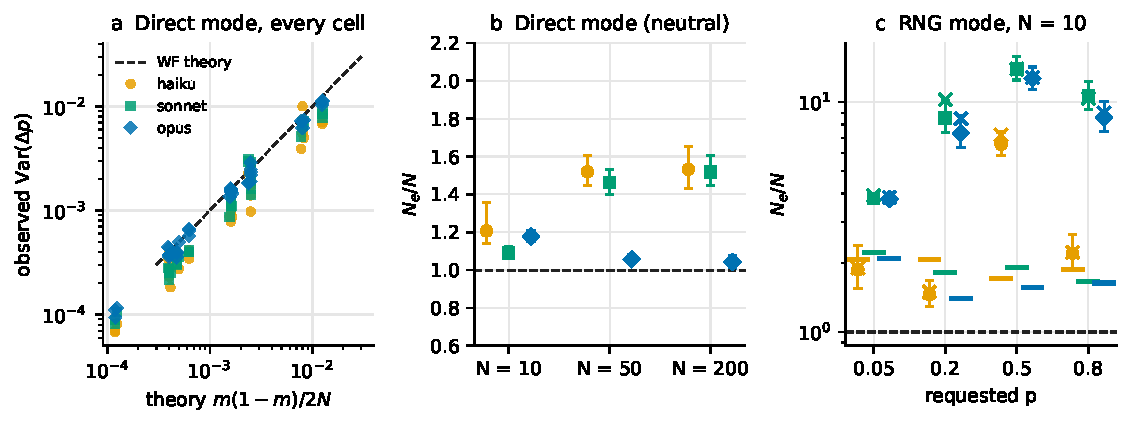
\includegraphics[width=\textwidth]{../figures/fig3_ne.pdf}
\caption{Variance of one-generation change. (a) Observed $\Var(\Delta p)$ in every direct-mode cell against the WF expectation (dashed line). (b) $\Ne/N$ in direct mode per model and $N$, with 95\% intervals from a call-level bootstrap. (c) RNG mode, $N=10$: $\Ne/N$ when each offspring copy uses one LLM bit requested at the current $p$; bars show the prediction of the first-order Markov model (Eq.~\ref{eq:rng}) and crosses the prediction from the full empirical autocorrelation function. Note the log scale in (c).}
\label{fig:ne}
\end{figure}

\subsection{Consequences over many generations}

\begin{figure}[t]
\centering
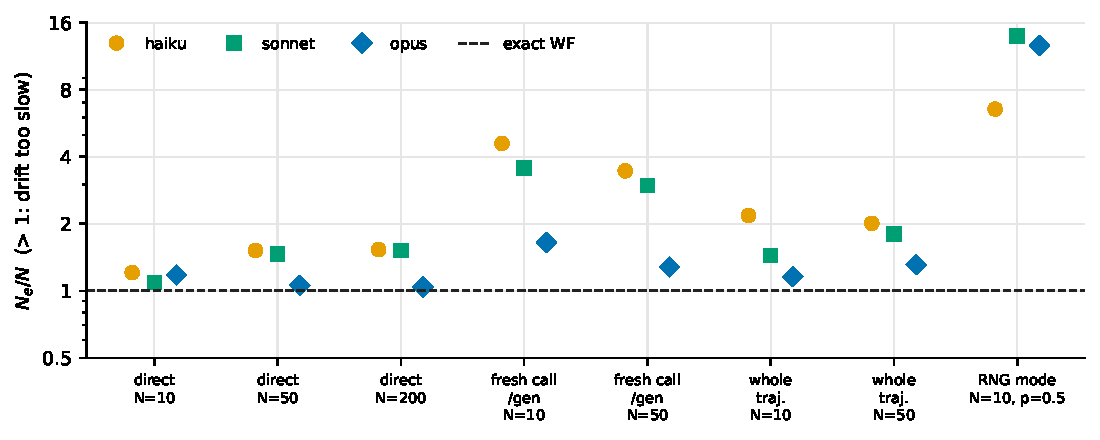
\includegraphics[width=\textwidth]{../figures/fig8_ne_by_mode.pdf}
\caption{$\Ne/N$ for each model across all modes (values in Table~\ref{tab:ne}). The dashed line is exact Wright--Fisher drift.}
\label{fig:modes}
\end{figure}

In multi-generation runs the shortfall in variance grew (Fig.~\ref{fig:modes}).
With a fresh call per generation, $\Ne/N$ at $N=10$ was \MlNeHaikuTen{} for Haiku, \MlNeSonnetTen{} for Sonnet and \MlNeOpusTen{} for Opus (at $N=50$: \MlNeHaikuFifty, \MlNeSonnetFifty, \MlNeOpusFifty).
Heterozygosity decayed accordingly (Fig.~\ref{fig:het}): after 40 generations at $N=10$ it was \MlHendHaikuTen{} for Haiku, \MlHendSonnetTen{} for Sonnet and \MlHendOpusTen{} for Opus, against \npHendTen{} in numpy WF and in theory.
Haiku's populations barely drifted at all.
None of its neutral populations starting at 0.5 or 0.8 fixed within 40 generations, while populations starting from a single copy were lost within a few generations; in numpy WF, \npFixHalfNeu{} of populations starting at 0.5 had fixed by then.
Sonnet fixed \MlFixSonnetHalfNeu{} and Opus \MlFixOpusHalfNeu{} (Fig.~\ref{fig:fix}a).
These differences come mainly from variance, not from a biased mean.
Regressing $\Delta p$ on $p-0.5$ gave slopes of \MlPullOpusTen{} (Opus), \MlPullSonnetTen{} (Sonnet) and \MlPullHaikuTen{} (Haiku) at $N=10$, a weak pull toward the middle for Haiku only, whereas the per-transition dispersion factor in the middle frequency range was \MlPhiMidHaiku{} (Haiku), \MlPhiMidSonnet{} (Sonnet) and \MlPhiMidOpus{} (Opus).
Fresh-call runs batched 40 populations per call, so they are not memoryless across populations, and their dispersion was lower than in direct mode, where one state was replicated 20 times.

When one call produced a whole trajectory, $\Ne/N$ was \WhNeHaikuTen{} (Haiku), \WhNeSonnetTen{} (Sonnet) and \WhNeOpusTen{} (Opus) at $N=10$.
These trajectories looked plausible at a glance (Fig.~\ref{fig:traj}), and every one of them stayed absorbed once it reached 0 or $2N$; \whBadLength{} of the \nWhTraj{} trajectories had the wrong length.
Their texture was wrong in a model-specific way.
Sonnet and Opus produced too many reversals: the lag-1 correlation of successive increments was \WhLagSonnetTen{} and \WhLagOpusTen, and the share of consecutive non-zero steps that changed direction was \WhRevSonnetTen{} and \WhRevOpusTen{}, against \npRevTen{} in numpy.
Haiku's trajectories were smoother instead (lag-1 correlation \WhLagHaikuTen, reversal rate \WhRevHaikuTen), with long monotone climbs and descents (Fig.~\ref{fig:traj}).
Whole trajectories also flattened the relation between starting frequency and fixation (Fig.~\ref{fig:fix}a): a single initial copy ($p_0=0.05$) went on to fix in \WhFixOpusFiveNeu{} (Opus) to \WhFixHaikuFiveNeu{} (Haiku and Sonnet) of trajectories by generation 40, against \npFixFiveNeu{} in numpy WF and an eventual probability of 0.05, while Haiku fixed only \WhFixHaikuEightyNeu{} of trajectories that started at 0.8 (numpy \npFixEightyNeu). These cells hold only 12 trajectories each, but the pattern suggests that in a single call the models tell stories in which rare alleles rise more often than chance allows.
Fresh-call trajectories had increment correlations close to zero (\MlLagOpusTen{} to \MlLagSonnetTen{} at $N=10$), as expected when each step is a separate call (Fig.~\ref{fig:dep}c).

\begin{figure}[t]
\centering
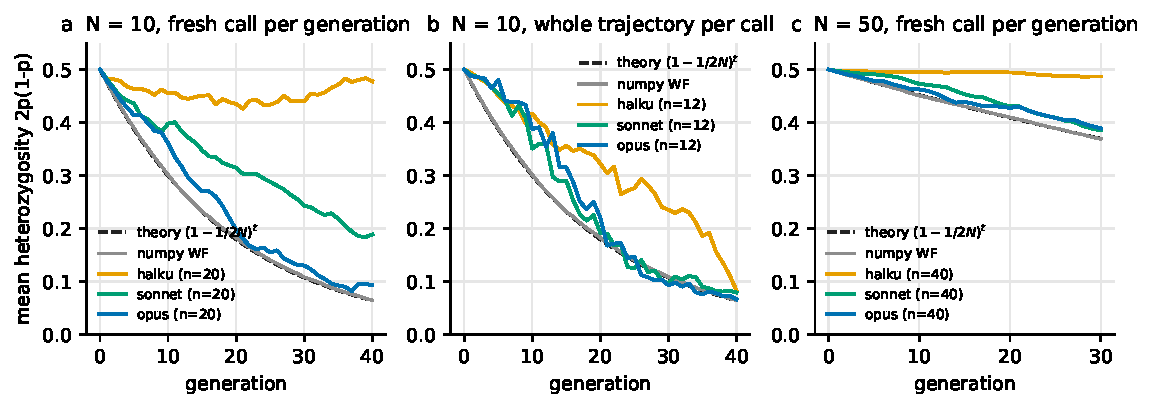
\includegraphics[width=\textwidth]{../figures/fig4_heterozygosity.pdf}
\caption{Mean heterozygosity $2p(1-p)$ over generations for populations starting at $p_0=0.5$, $s=0$, against theory (Eq.~\ref{eq:het} with $\Ne=N$) and 5,000 numpy WF replicates. $n$ is the number of LLM populations.}
\label{fig:het}
\end{figure}

\subsection{Selection}

All models moved frequencies in the favoured direction (Table~\ref{tab:sel}).
In fresh-call runs the effective selection coefficient estimated from all transitions was \MlSeffHaiku{} (Haiku), \MlSeffOpus{} (Opus) and \MlSeffSonnet{} (Sonnet), against \sTrueApprox{} for the WF expectation at the same states.
In whole-trajectory runs it was higher for every model, \WhSeffSonnet--\WhSeffHaiku, an exaggeration of \whSexMin--\whSexMax\%.
In single-generation direct mode the estimates rest on two calls per cell and were noisy; Haiku under-responded at $N=10$ (\dSeffHaikuTen) and Sonnet over-responded (\dSeffSonnetTen).
Because $\Ne/N>1$ as well, the product $\Ne s$ that governs fixation was inflated even where $s_{\mathrm{eff}}$ was right.
Fixation by generation 40 with $s=0.05$ (Fig.~\ref{fig:fix}b) nonetheless stayed close to the numpy values for Sonnet and Opus, possibly because slow drift also delays fixation within a fixed time window, so that the two errors partly cancel.
Haiku again fixed rarely (\MlFixHaikuHalfSel{} from $p_0=0.5$ against \npFixHalfSel{} in numpy).

\begin{table}[t]
\centering\small
\caption{Effective selection coefficient for a stated $s=0.05$. Direct mode: mean over cells of $(\bar p'-p)/[p(1-\bar p')]$. Trajectory modes: regression of $\Delta p$ on $p(1-p)$ over all polymorphic transitions; the WF expectation at the same states is \sTrueApprox.}
\label{tab:sel}
\begin{tabular}{lccccc}
\toprule
 & \multicolumn{3}{c}{direct, one generation} & fresh call/gen. & whole trajectory \\
\cmidrule(lr){2-4}
Model & $N=10$ & $N=50$ & $N=200$ & $N=10$ & $N=10$ \\
\midrule
Haiku & 0.016 & 0.032 & 0.043 & 0.045 & 0.072 \\
Sonnet & 0.104 & 0.076 & 0.054 & 0.065 & 0.064 \\
Opus & 0.046 & 0.041 & 0.051 & 0.052 & 0.069 \\
\bottomrule
\end{tabular}

\end{table}

\begin{figure}[t]
\centering
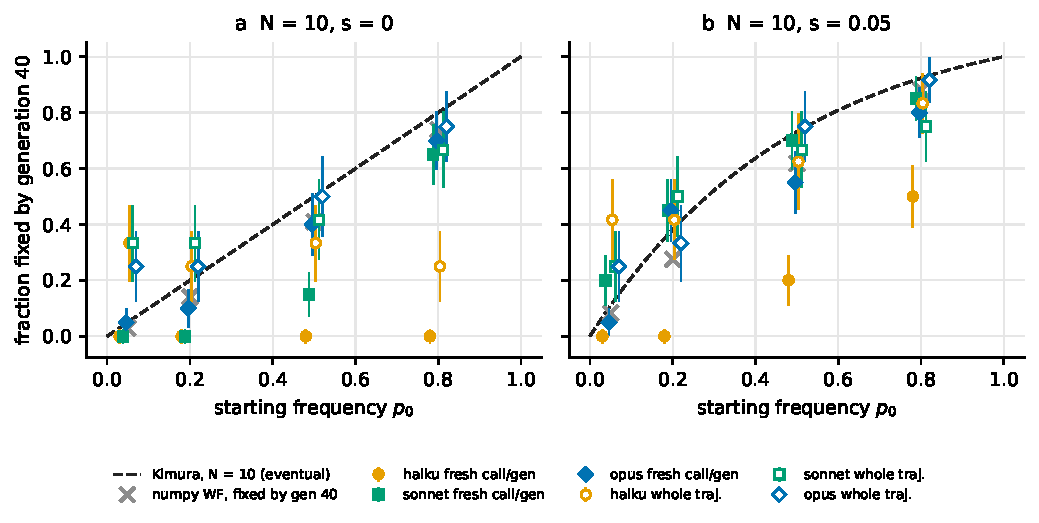
\includegraphics[width=\textwidth]{../figures/fig5_fixation.pdf}
\caption{Fraction of $N=10$ populations fixed by generation 40 against starting frequency, without (a) and with (b) selection. Filled symbols: fresh call per generation (20 populations per point); open symbols: whole trajectory per call (12 per point). Error bars are binomial standard errors. Grey crosses: numpy WF truncated at the same generation. Dashed lines: eventual fixation probability ($p_0$, or Kimura's formula with $\Ne=N$).}
\label{fig:fix}
\end{figure}

\begin{figure}[t]
\centering
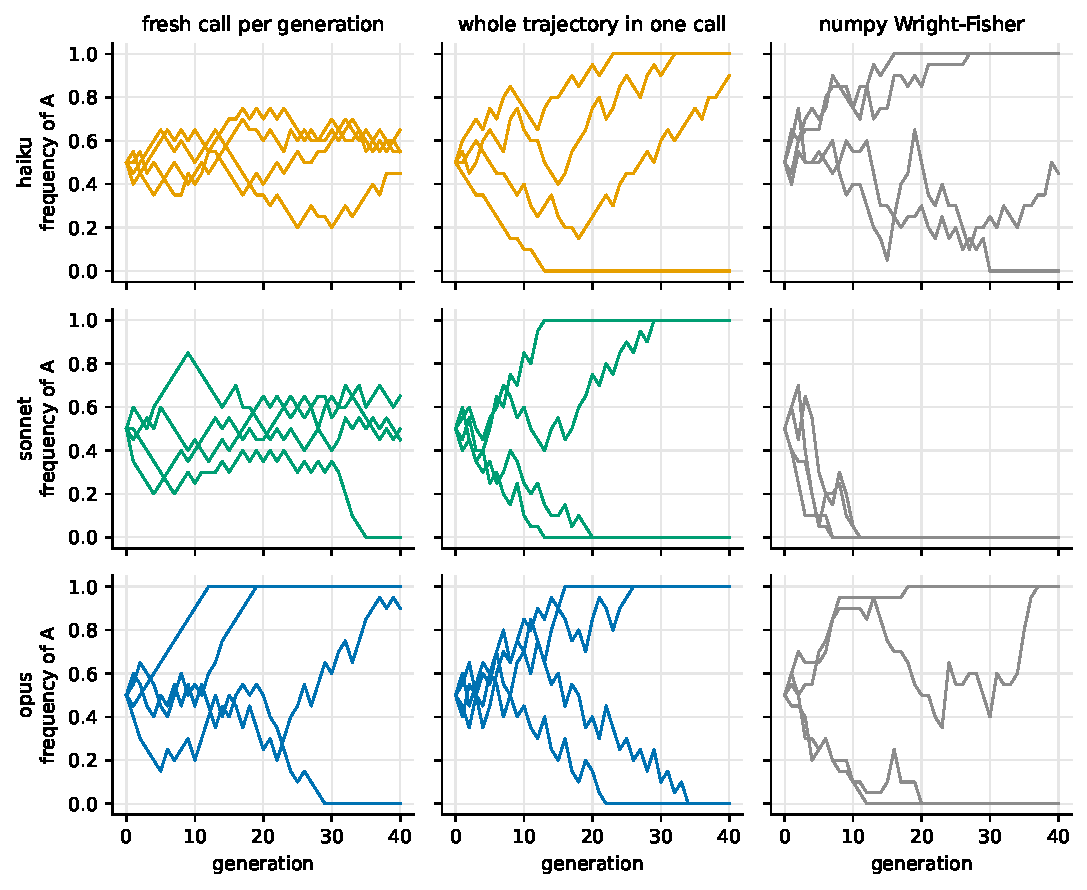
\includegraphics[width=0.92\textwidth]{../figures/fig6_trajectories.pdf}
\caption{Example trajectories at $N=10$, $p_0=0.5$, $s=0$: four populations from fresh-call runs, four from one whole-trajectory call, and four numpy WF replicates per row.}
\label{fig:traj}
\end{figure}

\subsection{RNG mode: bad randomness without a model of the process}

When LLM bits drove an otherwise exact WF step, drift was much too slow (Fig.~\ref{fig:ne}c).
With one bit per offspring copy and $N=10$, $\Ne/N$ at $p=0.5$ was \rngNeHaikuHalf{} (Haiku), \rngNeSonnetHalf{} (Sonnet) and \rngNeOpusHalf{} (Opus), and at $N=50$ it was \rngNeHaikuHalfFifty, \rngNeSonnetHalfFifty{} and \rngNeOpusHalfFifty.
The first-order Markov model of Eq.~\eqref{eq:rng}, with the fitted $\rho$, predicted only \rngMarkovOpusHalf--\rngMarkovSonnetHalf.
A prediction from the full empirical autocorrelation function, which includes the negative correlations at lags 2 and 4 and beyond, matched the observed values at $N=10$ to within \rngAcfMaxDev\% (\rngAcfHaikuHalf, \rngAcfSonnetHalf, \rngAcfOpusHalf).
The LLM bits are balanced over windows of tens of digits, so the sum of 20 bits varies far less than a binomial count.
At $p=0.2$ and $p=0.05$ the excess was smaller but still present for $N=10$ (\rngNeHaikuTwenty--\rngNeSonnetTwenty{} at $p=0.2$).
For larger windows at $p\neq0.5$ the estimate fell below 1 for some models, because windows then spanned several calls whose overall frequencies differed; the between-call heterogeneity adds variance that the within-call balancing removes.
Exaggeration of $p$ also gave a systematic $\E[\Delta p]=\pi-p$ that pushed rare alleles further down and common ones further up, which in a multi-generation run acts like positive frequency dependence.

Converting fair LLM bits into Bernoulli($p$) draws with the comparison method gave only \fcNHaiku--\fcNOpus{} complete $N=10$ trajectories per model, so these numbers are rough.
None of them fixed (all were lost), and their $\Ne/N$ was \fcNeHaiku--\fcNeOpus.
A Markov chain fitted to the same bits, run for 3,000 trajectories, fixed in only \fcSurFixOpus--\fcSurFixSonnet{} of cases instead of 0.5.
The comparison method maps alternation bias into a probability error that depends on the binary expansion of $p$, so a correlated bit source does not just add noise but introduces a directional force.

\begin{figure}[t]
\centering
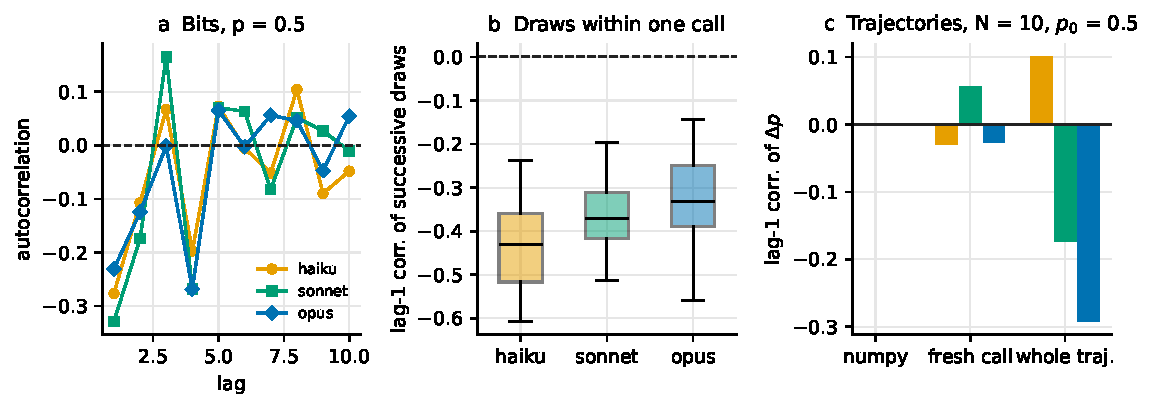
\includegraphics[width=\textwidth]{../figures/fig7_dependence.pdf}
\caption{Dependence. (a) Autocorrelation of bits at $p=0.5$ by lag (pooled within calls). (b) Lag-1 correlation of successive draws within direct-mode calls, one value per cell. (c) Lag-1 correlation of successive increments $\Delta p$ in trajectories at $N=10$, $p_0=0.5$; numpy WF gives zero.}
\label{fig:dep}
\end{figure}

\subsection{Model comparison}

A larger model was not uniformly a better random source.
Opus was the closest to WF behaviour in every mode where the model simulates the process (Table~\ref{tab:ne}; direct $\Ne/N$ \dNeOpusFifty--\dNeOpusTen, fresh-call \MlNeOpusFifty--\MlNeOpusTen, whole trajectory \WhNeOpusTen--\WhNeOpusFifty), and Haiku was the furthest.
Sonnet sat in between in the trajectory modes but matched Haiku in direct mode at $N\ge50$.
The ranking does not hold for raw bits.
Opus bits alternated slightly less than the others, yet in RNG mode they slowed drift as much as Sonnet's (\rngNeOpusHalf{} against \rngNeSonnetHalf{}, Haiku \rngNeHaikuHalf), and Opus was the most repetitive across calls.
All three models exaggerated probabilities to a similar degree.

\section{Discussion}

The answer to the question in the title is no, at least for the models we tested.
When an LLM is the random number source, drift runs too slowly.
In population-genetic terms the LLM behaves like a population that is larger than stated, \dNeMin{} to \dNeMax{} times larger when a single state is resampled, \trajNeMin{} to \trajNeMax{} times larger in multi-generation simulations, and \rngNeMin{} to \rngNeMax{} times larger when its bits are used directly as a random source.

The error has the same root as the human biases described for random sequence generation \citep{wagenaar1972generation,falk1997making}.
Over-alternation and the avoidance of long runs make sums of LLM bits less variable than binomial sums.
When the model produces counts directly, it builds batches of draws that look like a correct sample, spread around the right mean but too tightly and too evenly.
Earlier work found the same over-alternation in LLM coin flips \citep{koevering2024random} and too little spread across simulated individuals \citep{aher2023using}; what we add is that these errors translate into a quantifiable change in $\Ne$, and through it into slower loss of heterozygosity, delayed fixation and a stronger effect of selection.

Two results were not what a simple model predicted.
First, the models did not hedge toward one half when asked for a biased coin; they made rare events rarer.
This differs from a probability-weighting view in which small probabilities are overweighted, and it matters for population genetics because a source that under-produces rare outcomes pushes rare alleles toward loss.
Second, a first-order Markov model with the measured alternation rate underestimated the effect of the bits on drift by a factor of up to \markovUnderFactor.
LLM bit strings are balanced over long windows, not just from one digit to the next, so only a model that uses the full autocorrelation function accounts for the variance of their sums.
This is a warning against summarising LLM randomness by a single alternation statistic.

The comparison between modes separates two failures.
In RNG mode the model does not know about the population at all, yet drift is still distorted, so poor randomness on its own is enough to bias the outcome.
In direct mode the model knows the process, uses the right mean and the right direction of selection, and errs mainly in the variance.
Its errors are smaller than in RNG mode because it is not composing outcomes digit by digit; it behaves as if it knew roughly how much a binomial count should vary and then compressed that spread.
The memory experiment did not support the idea that LLMs imagine drift as smooth.
Sonnet and Opus trajectories reversed direction too often, and only Haiku produced overly smooth paths.
When each generation was a fresh call, the increments were uncorrelated but too small, so memory changes the texture of trajectories more than their overall rate.

For applied work the conclusions are practical.
LLM agents in evolutionary or ecological simulations should draw their random numbers from a proper pseudo-random generator, passed in through the prompt or a tool, as recent work also suggests \citep{gu2026stochasticity}.
If an LLM must generate stochastic outcomes, its effective $\Ne$ should be measured with checks like ours before the results are interpreted.
Batching, phrasing and model choice all change the size of the error, and identical or near-identical prompts produce correlated answers across calls, so replicate simulations are not independent replicates.

\section{Limitations}

Every LLM call ran as a subagent inside an agent harness, with a large system prompt and tools available that the model was told not to use.
We could not set the sampling temperature, which is known to affect LLM coin flips \citep{koevering2024random}, and all calls used low reasoning effort.
We tested three models of one family at one point in time, so the numbers will not transfer directly to other models or versions.
The multi-generation part of the grid was trimmed to $N=10$ and $N=50$, the number of populations per cell was small (12 to 40), and fixation was measured at a fixed horizon rather than at absorption.
The fresh-call runs batched up to 40 populations in one call and the direct-mode calls asked for 20 draws at once, so they test batched randomness; the first-draw analysis shows that batching itself creates dependence, but a design with one draw per call would cost twenty times more calls.
Run codes made replicate prompts differ, but they may themselves act as seeds and their effect was not varied systematically.
In RNG mode the windows of bits for large $N$ crossed call boundaries, which mixes within-call balance with between-call heterogeneity, and the multi-generation fair-coin runs contain only 8 to 12 trajectories per model.
Finally, our parametric models are descriptive: the dispersion factor $\phi$ summarises the output but does not explain how the model generates it.

\section*{Data and code availability}
All prompts, raw responses, scripts, results and figures are in the project repository (\url{https://github.com/sarabehnamian/LLM-random-drift}).
\texttt{data/raw/calls.jsonl} holds one record per LLM call with its prompt, response, timing and model family; \texttt{data/raw/memoryless/} holds the fresh-call trajectories; \texttt{src/design.py} generates the calls, \texttt{src/ingest.py} extracts them from the agent transcripts, \texttt{src/analysis.py}, \texttt{src/figures.py} and \texttt{src/summary.py} produce every number, figure and table in this paper, and \texttt{theory/} contains the derivations and their numerical checks.

\bibliographystyle{plainnat}
\bibliography{references}

\end{document}
